% Section 2 - The mapping problem
% Roberto Masocco <roberto.masocco@uniroma2.it>
% June 5, 2024

% ### The mapping problem ###
\section{The mapping problem}
\graphicspath{{figs/section2/}}

% --- The mapping problem ---
\begin{frame}{The mapping problem}{Definition}
  Using \textbg{exteroceptive sensors}, a robot can gather information about the environment, which can be used to build a \textbg{map} of it.\\
  \bigskip
  A \textbg{map} is a \textbg{representation} of the environment, in a format that the robot can \textbg{understand}, \textbg{parse}, and \textbg{store}.\\
  \bigskip
  The utimate goal of mapping is twofold:
  \begin{itemize}
    \item to enable the robot to \textbg{localize itself} within the environment;
    \item to enable \textbg{safe navigation} of the robot within the environment.
  \end{itemize}
\end{frame}
\begin{frame}{The mapping problem}{Challenges}
  Given the utility requirement of a map, the mapping problem must be \textbg{continuously solved in real time}.\\
  \medskip
  Thus, it is challenging because:
  \begin{itemize}
    \item routines must be \textbg{efficient}, and run at a sufficiently \textbg{high rate};
    \item the map must be \textbg{accurate}, and \textbg{reliable};
    \item the map must be in a format that is as much \textbg{easy to load and parse} as possible, taking up as little \textbg{memory} as possible;
    \item the map must stay \textbg{up-to-date}, and \textbg{consistent} with the environment.
  \end{itemize}
\end{frame}
\begin{frame}{The mapping problem}{Tools for the job}
  The most important tool for the mapping problem is the \textbg{occupancy grid}, a representation of the environment as a \textbg{grid} of \textbg{cells}, each of which is \textbg{occupied} or \textbg{free}.\\
  \bigskip
  The occupancy grid is a \textbg{probabilistic} representation, where each cell is associated with a \textbg{probability} of being occupied or free.\\
  \bigskip
  The occupancy grid is usually built using \textbg{LiDAR} or \textbg{camera} depth data, and is updated in real time as the robot moves.\\
  \bigskip
  The occupancy grid is the most common representation for \textbg{local} and \textbg{global} maps.\\
  \bigskip
  To efficiently store an occupancy grid, \textbg{tree-like data structures} are often employed (\emph{e.g.}, \textbg{octrees}).
\end{frame}
\begin{frame}{The mapping problem}{Tools for the job}
  The second most important class of tools are \textbg{navigation algorithms}, which use the map to plan a \textbg{safe} and \textbg{efficient} path for the robot to follow.\\
  \bigskip
  The definition of such algorithms involves \textbg{geometry}, as well as \textbg{optimization} and \textbg{search} techniques.\\
  \bigskip
  They usually rely on two mathematical subjects:
  \begin{itemize}
    \item \textbg{topology}, to define the \textbg{connectivity} of the map (\emph{e.g.}, Voronoi tessellation);
    \item \textbg{graph theory}, to define the \textbg{best way} of moving from one free cell to another (\emph{e.g.}, Dijkstra's, A$^\star$ algorithms).
  \end{itemize}
\end{frame}
\begin{frame}{The mapping problem}{Tools for the job}
  \begin{figure}
    \centering
    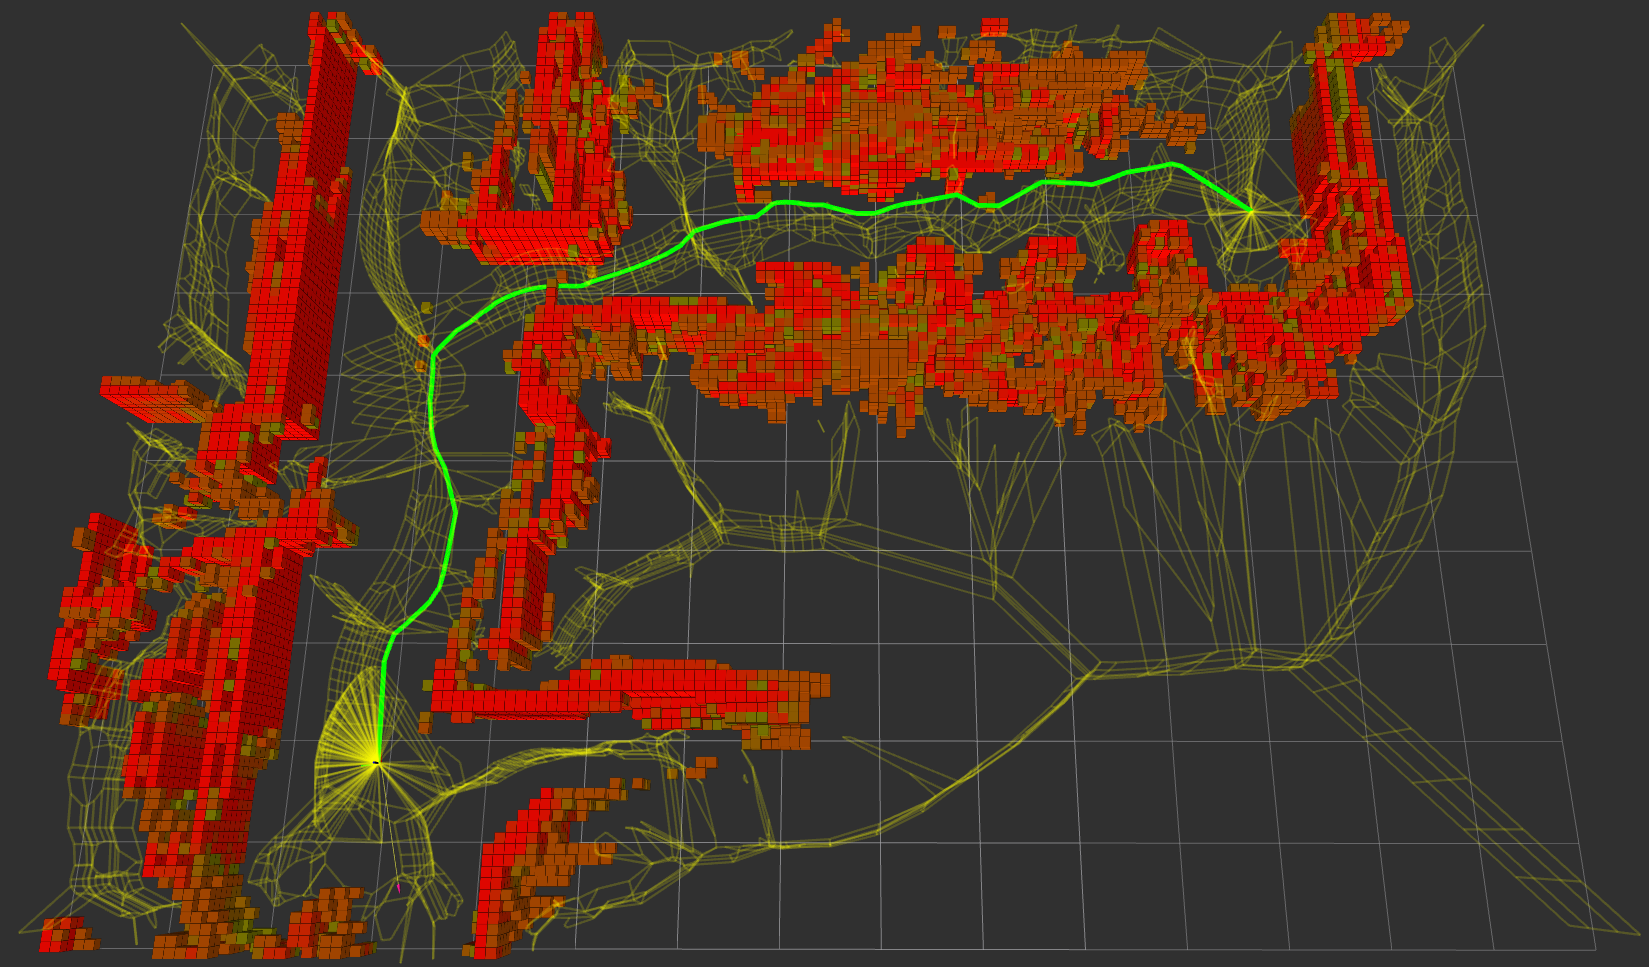
\includegraphics[width=.65\textwidth]{navigation_stack}
    \caption{Mapping and navigation algorithms execution.}
    \label{fig:navstack}
  \end{figure}
\end{frame}
